\documentclass[11pt]{article}
\usepackage[utf8]{inputenc}
\usepackage{graphicx}
\graphicspath{ {images/} }
\usepackage{amsmath}
\usepackage{placeins}
\usepackage{multirow}

\title{Coursework 1 – Transient Conduction}
\author{Adam Duncan}
\date{\today}

\begin{document}

\maketitle

\section{\emph{Part A: Using lumped capacitance}}
\subsection{Assumptions}
\begin{itemize}
	\item Internal temperature of the steel ball is uniform at any time t.
	\item No change in water temperature.
	\item No heat transfer by radiation.
	\item Material is standard carbon steel.
	\item Material properties are constant (taken at average temperature $T = 469 ^{o}C$).
\end{itemize}
\subsection{Properties}
\begin{table}[h]
	\centering
	\caption{Properties from problem}
	\begin{tabular}{lllll}
		Property & Value & Unit &  &  \\ \cline{1-3}
		Characteristic   length, L & 5 & cm &  &  \\
		Diameter, D & 10 & cm &  &  \\
		Temperature   of the water, $T_w$ & 38 & $^oC$ &  &  \\
		Initial   temperature of steel ball, $T_{s,1}$ & 900 & $^oC$ &  &  \\
		Final   temperature of steel ball, $T_{s,2}$ & 200 & $^oC$ &  &  \\
		Heat transfer   coefficient, h & 600 & $W/m^{2}K$ &  & 
	\end{tabular}
	\label{tab1}
\end{table}

\begin{table}[h]
	\centering
	\caption{Properties from literature}
	\begin{tabular}{llll}
		Property & Value at $T_{avg}$(469 $^{o}C$) & Unit & Source \\ \hline
		Specific heat   capacity, Cp & 552 & $J\cdot kg^{-1} K^{-1}$ & \cite{jean-marc_franssen_fire_2015} \\
		Density, $\rho$ & 7.8 x $10^3$ & $kg\cdot m^{-3}$ & \cite{bergman_fundamentals_2011} \\
		Conductivity, $k$ & 40 & $W\cdot m^{-1} K^{-1} $& \cite{jean-marc_franssen_fire_2015}
	\end{tabular}
	\label{tab2}
\end{table}
\FloatBarrier

The density of steel is assumed to be constant over the temperature range so the value in table \ref{tab2}, which is given at 300K, is assumed to be accurate. To confirm this assumption is acceptable the elongation was calculated using the ISO 834 standard equations\cite{jean-marc_franssen_fire_2015}. This showed the overall change in volume of the sphere was ~3\% over the full temperature range of the problem. As $V \propto \rho$ this change is low enough to be discounted and for the assumption to be justified.

\begin{table}[h]
	\centering
	\caption{Properties error analysis}
	\begin{tabular}{lllll}
		T [$^{o}C]$ & $C_{p}$ [$J \cdot kg^{-1}K^{-1}$] & $\Delta$\% from $T_{469}$ & k [$W \cdot m^{-1}K^{-1}$] & $\Delta$\% from $T_{469}$ \\ \hline
		900 & 650 & 56 & 27.3 & -29 \\
		469 & 416 & 0 & 38.4 & 0 \\
		38 & 454 & 9 & 52.7 & 37
	\end{tabular}
	\label{tab3}
\end{table}

Similarly the variation in specific heat capacity ($C_p$) and conductivity ($k$) were considered over the full temperature range as shown in Table \ref{tab3}. The value of $k$ varies from the $T_{mean}$ value by roughly $\pm 30\%$  but the $T_{mean}$ value is only $4\%$ different from the mean of values of $k$ at the two temperature extremes. This fact coupled with the information given in ISO 835 standard \cite{jean-marc_franssen_fire_2015} suggest a linear change in $h$, which makes the approximation useful. 

The variation in $C_p$ is less clear cut, with the value at $T_{mean}$ falling much closer to the value at $T_{38}$ than the value at $T_{900}$ as showing in Table \ref{tab3}. This variation is due to the non-linear variation of $C_p$ with temperature \cite{jean-marc_franssen_fire_2015}. Further investigation would be needed get an accurate estimate of the level of error this approximation introduces to the result but this falls beyond the scope of this problem set so the approximation is used as a best estimate.
\pagebreak
\subsection{Schematic}
\begin{figure}[!htbp]
	\centering
	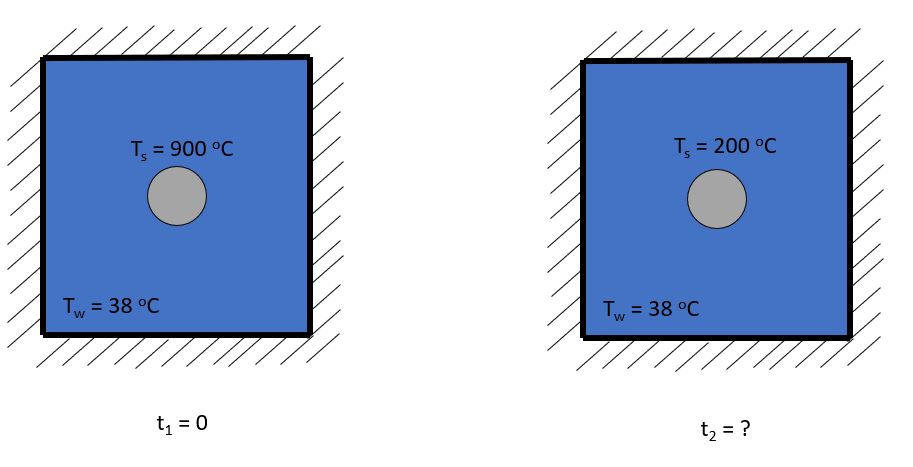
\includegraphics[width=0.85\textwidth]{part_a_fig}
	\caption{Part A schematic at initial and final state.}
	\label{fig:schem_a}
\end{figure}
\FloatBarrier
\subsection{Analysis}

Energy balance for closed system gives the following equation.
\begin{equation}\label{eqn_1}
	\stackrel{.}{Q} = hA(T_{s}-T_{f}) = C_{p}\rho V \frac{dT_{c}}{dt}
\end{equation}

Where $\stackrel{.}{Q}$ is heat [$W$], $h$ is the heat transfer coefficient [$W/m^{2}K$], $A$ is the surface area between the ball and water [$m^{2}$], $T_{s}$ is the temperature of the steel ball [$^{o}C$], $T_{f}$ is the temperature of the water [$^{o}C$], $C_{p}$ is the specific heat capacity [$J/mK$], $\rho$ is the density of the steel ball[$kg/m^{3}$], $V$ is the volume of the steel ball [$m^3$] and $t$ is the time [$s$].
\newline

Rearranging (\ref{eqn_1}) to separate the variables gives.
\begin{equation}\label{key}
	\frac{1}{T_{s}-T_{f}} dT_{c} = \frac{hA}{C_{p}\rho V}dt
\end{equation}

Which integrates to give.
\begin{equation}\label{eqn_3}
	\ln{(\frac{T_{s1}-T_{f}}{T_{s2}-T_{f}})} =  \frac{hA}{C_{p}\rho V}(t_{2}-t_{1})
\end{equation}
Where $t_{i}$ and $T_{si}$ are the time [s] and temperature [$^oC$] at state $i$ receptively.

Rearranging (\ref{eqn_3}) to make $t_{2}$ the subject gives.
\begin{equation}\label{key}
	t_{2} = \frac{C_{p}\rho V}{hA}(\ln{(\frac{T_{s1}-T_{f}}{T_{s2}-T_{f}})})
\end{equation}

Substituting in the values for the variables given in Tables \ref{tab1} and \ref{tab2} gives the final value.
\boldmath
\begin{equation}\label{t1}
	t_2 = 200 s
\end{equation}
\unboldmath
Where $t_2$ is the time for the steel ball to reach a temperature of $200^{o}C$ under given assumptions.

\section{\emph{Part B: Lumped capacitance justification}}
The lumped capacitance method is only valid if the ratio of the conductive heat transfer to convective heat transfer is low. This ratio is known as the Biot number, $Bi$, and is given by.
\begin{equation}\label{eqn_biot}
	Bi = \frac{h \cdot L_{c}}{k}
\end{equation}
Where $h$ is convective coefficient [$W/m^{2}K$], $L_{c}$ is the characteristic length [m] and $k$ is the conductivity [$W/m \cdot K$]. 

Applying the values from Tables \ref{tab1} and \ref{tab2}, choosing to set $L_{c}=R$ and substituting into equation (\ref{eqn_biot}) gives:
\begin{equation}\label{biot_num}
	Bi = 0.7
\end{equation}

If $Bi > 0.1$ then the lumped capacitance method is no longer applicable as the assumptions made introduce non-trivial errors \cite{bergman_fundamentals_2011}. This means that the result in part A is likely inaccurate.

It is worth noting that the choice of $L_c$ is significant. It is common to select $L_c$ to be the maximum distance over which a temperature gradient would occur, as has been done above, but the method from the mathematical derivation uses $L_c = \frac{V}{A_s}$ which for a sphere gives $L_c = \frac{R}{3}$. This means the use of $L_c = R$ will tend to overestimate the value of $Bi$. In this case however, using $L_c = \frac{R}{3}$ gives $Bi = 0.25$ so the result can still be assumed to be inaccurate using the lumped capacitance method despite the overestimate.

\section{\emph{Part C: Transient conduction}}
\subsection{Assumptions}
\begin{itemize}
	\item No change in water temperature.
	\item No heat transfer by radiation.
	\item Material is standard carbon steel.
	\item Material properties are constant (taken at average temperature $T = 469 ^{o}C$).
\end{itemize}
\subsection{Time interval to cool centre of sphere to $200 ^{o}C$}
As the initial and final temperature of the sphere are specified as well as the temperature of the fluid which is assumed to be constant, the ratio below can be calculated.
\begin{equation}\label{ratio_1}
	\frac{T_{(0,t)} -T_{f}}{T_{i} - T_{f}}
\end{equation}
Using the values in Table \ref{tab1} the answer to (\ref{ratio_1}) is $0.19$. Taking the inverse of (\ref{biot_num}) gives $1.33$. These two values allow the Fourier number to be determined from the Heisler chart \cite{multidimensional-transient}, which is determined to be.
\begin{equation}\label{Fr_1}
	Fo = 0.67
\end{equation}
The Fourier number is defined below.
\begin{equation}\label{Fr_2}
	Fo = \frac{tk}{\rho C_{p} R^{2}}
\end{equation}

Using the result from (\ref{Fr_1}) and substituting in the values from Tables \ref{tab1} and \ref{tab2} into (\ref{Fr_2}) gives the final result time taken.
\boldmath
\begin{equation}\label{t2}
	t = \frac{F_{o}\rho C_{p} R^{2}}{k} = 182 s
\end{equation}
\unboldmath

Comparing this result and (\ref{t1}), the result gained from the lumped capacitance method, it can be seen the two are of a similar magnitude but (\ref{t2}) is lower than (\ref{t1}). This matches with expectations as the assumptions used in section 1 were found to be near the boundary so the error introduced by applying them would be significant but still give an answer of the same magnitude. Where it differs from expectation is that the temperature gradient that was found to be important for this case in section 2 should take additional time to reach the centre point so the transient response would be expected to take longer to reach the target temperature than the lumped capacitance method. The fact that this is not the case here may be attributed to errors introduced by the approximations mentioned in section 1 and errors from reading from Heisler charts.

\subsection{Time interval to cool surface of sphere to $200 ^{o}C$}
To find the centre temperature of the sphere when the surface reaches $200 ^{o}C$ a quantification of the temperature gradient is needed. The Heisler charts can again be used to find this using $\frac{1}{Bi}=1.33$ and that $\frac{r}{r_{0}}= 1$ for this example, giving the following.
\begin{equation}\label{surf_2_cent}
	\frac{T - T_{\infty}}{T_{c}-T_{\infty}} = 0.65
\end{equation}

Where $T$ is the surface temperature [$^{o}C$], $T_{\infty}$ is the water temperature [$^{o}C$] and $T_c$ is the centre temperature [$^{o}C$].

Rearranging (\ref{surf_2_cent}) and using the temperatures in Table \ref{tab1} gives.

\begin{equation}\label{cent_temp}
	T = 287 ^{o}C
\end{equation}

Applying this to (\ref{ratio_1}) and again using the $\frac{1}{Bi}=1.33$ result allows the Fourier number to be found from the Heisler chart \cite{bergman_fundamentals_2011}.
\begin{equation}\label{fo_2}
	Fo = 0.42
\end{equation}

Substituting (\ref{fo_2}) into (\ref{Fr_2}) gives the final result.
\begin{equation}\label{t3}
	t = 114s
\end{equation}

It makes intuitive sense that (\ref{t3}) is lower than (\ref{t2}) as the surface will cool faster then the centre.

\section{\emph{Part D: Non-infinite water bath}}
If the tub of water is non-infinite it is possible to quantify how the temperature of the water will change during the process to check if the assumption of constant temperature is valid. 

From the Heisler charts it is possible to find the proportion of total heat the steel contains that has dissipated at a given time. The temperature rise of the tank of water (Figure \ref{fig:schem_d}) when the centre of the steel ball has reached $200^{o}C$ is considered here.
\begin{figure}[!htbp]
	\centering
	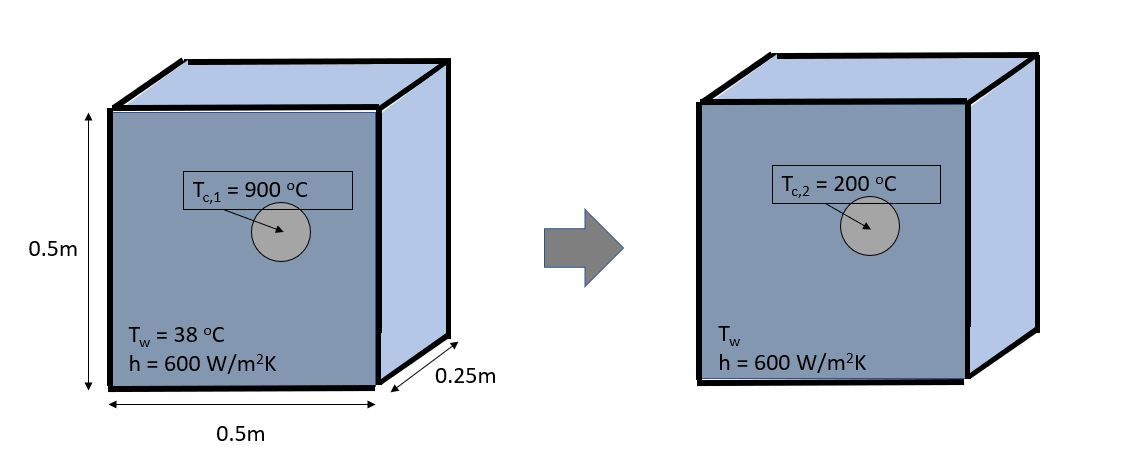
\includegraphics[width=0.85\textwidth]{part_d_fig}
	\caption{Part D schematic at initial and final state.}
	\label{fig:schem_d}
\end{figure}

Using the results of (\ref{biot_num}) and (\ref{Fr_1}) and referencing the Heisler chart \cite{bergman_fundamentals_2011} it is possible to calculate the following.
\begin{equation}\label{q_ratio}
	\frac{Q}{Q_o} = 0.7
\end{equation}
Where $Q$ is the heat transferred at time t [W] and $Q_o$ is the total heat stored initially in the steel ball [W].

$Q_o$ can be calculated simply.
\begin{equation}\label{q_o}
	Q_o = \rho_s C_{p,s} V_s T_{c,1}
\end{equation}
Where $\rho_s$ is the density of steel,$C_{p,s}$ is the heat capacity of steel, V is the volume of the steel ball [$m^3$] and $T_{c,1} $is inital temperature 900$^oC$.

Given the continued assumption that no heat is via the sides of the water tank all the heat, $Q$, that leaves the steel ball is absorbed by the water, shown in the following expression.

\begin{equation}\label{q}
	Q = \rho_w C_{p,w} V_w \Delta T_{w}
\end{equation}

Where the variables are the same as (\ref{q_o}) but for water, denoted by the subscript $w$ on each.

Substituting (\ref{q}) and (\ref{q_o}) into (\ref{q_ratio}), rearranging to make $\Delta T_w$ the subject and using the known values shown in Figure \ref{fig:schem_d} gives.
\begin{equation}\label{delta_t}
	\Delta T_w = 5.4 ^oC
\end{equation}

Doing the same analysis using the $Fo$ number for the surface reaching $200^oC$ and using the assumptions detailed in the lumped capacitance method give values of $\Delta T_w$ of $\pm1^oC$, so the temperature change is similar for all examples.

This is a 14\% change in the temperature and a more in depth analysis would look at the change in water properties over a $5^oC$ temperature rise to quantify this further.

\FloatBarrier
\section{\emph{Part E: Equilibrium temperature}}

\bibliographystyle{plain}
\bibliography{refs}
\end{document}

